
\chapter{人脸多属性属性识别的架构}
本章主要介绍人脸属性识别任务数据库和一些人脸属性识别中常用的方法,并且根据这些方法的弱点和问题,提出改进方法改进并进行实验。包括人脸属性中输入图片对于识别效果的影响,改进网络结构对于属性性能的提升,设计面向多数据分布和多属性分类的神经网络框架、以及对于网络输出置信度模块的构建。
\section{人脸属性性质分析}
\subsection{人脸属性的类别}
人脸属性的数据标注的环境各有不同限制性场景和非限制性场景(如固定摄像头拍摄和日常采集的场景),其中标签往往具有很多种表示和性质,比如相对性标注和绝对属性标注(如颜值数据标注之间只有相互的高低,但没有绝对的属性标签)但总体分为有序性与无序性,整体性与局部性等\cite{HUHAN_HETER},具体包括:
\begin{enumerate}
\item 无序性:
无序性的属性有两个或两个以上的类别(值),但在类别之间没有内在的顺序。 例如,种族是具有多个类别的名义属性,例如黑色,白色,亚洲等,并且这些值(类别)没有内在排序。;
\item 有序性:有序性的属性具有明确的变量排序。 例如,一个人的年龄,通常从0到100,是不平均的。(实际上,年龄不仅是相互独立的存在,在不同的年龄标签中,具有一定钟形的分布)
\item  整体性:
整体性标签描述了整个人脸的特征,诸如年龄,性别,种族等;
\item 局部性:
和整体性标签相反,局部性描述了部分人脸的特征,例如:尖鼻子,大嘴唇等。
\end{enumerate}
本文中也主要根据上面的人脸属性的性质来设计网络和分析问题。
\subsection{多属性标签表示形式}
在训练的过程中,人脸属性通常以分类或者回归问题的形式出现,但是在多属性识别的任务中,通常使用标签编码或者多标签回归的方式。

方法一:标签编码:
将多属性标签组合进行编码(比如,将一岁亚洲男性标记为001,将一岁非洲男性标记为002等),将多属性问题转化为分类编码问题,也就是单一属性。

方法二:多标签回归
通过回归的方法,使预测的特征向量与Groud-truth属性向量的损失越来越小,二者趋向接近,由此得到预测的特征向量。

\subsection{属性之间的相互联系}
\begin{figure}[!ht]
 \centering
	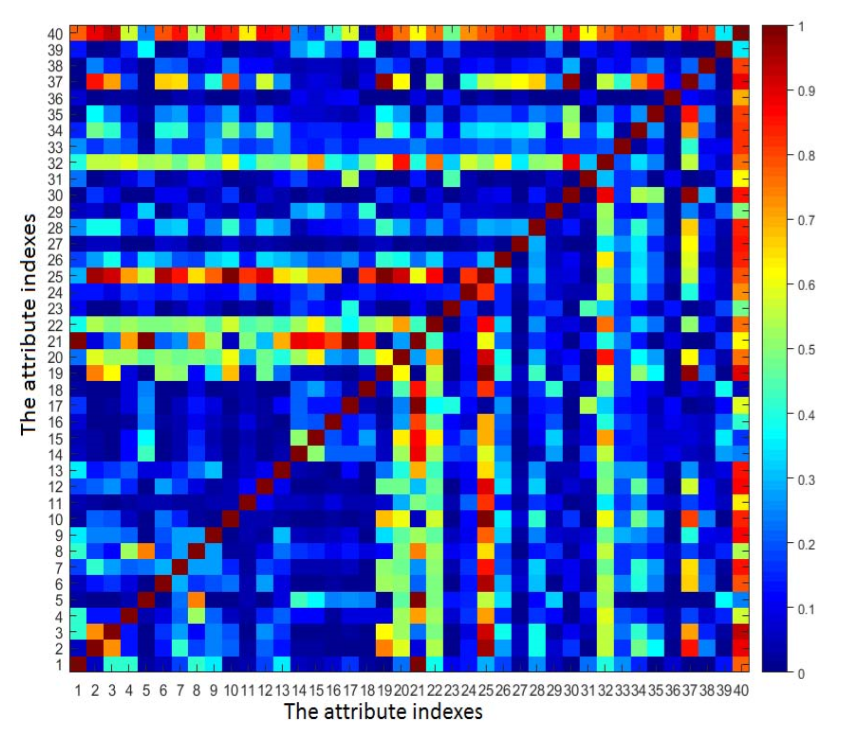
\includegraphics[width=4.0in]{attrconv.png}
	\caption{人脸属性之间的相互联系}
\end{figure}


正如上文提到的,很多人脸属性其实并没有关系,具有非常大的异构性,比如比如头发长短和是否微笑是没有必然关系的,而年龄是可量化的,而种族是类别化的,在表达方式上就是不一样的,这就需要不同的处理方式,也是为什么要把人脸属性作为一个multi-task的场景来处理的基本原因。

但是作为人脸特征,它们同时在很多表现过程之中,也有很多共同的地方。
通过对CelebA数据集的40个属性做了成对的Co-occurrence计算,它揭示了,属性的相关性是普遍存在的,比如性别男女和是否有胡子和头发长短是具有很强的相关性,我们认为它对属性学习有所帮助。因为属性之间具有相关性也就意味着所使用的表示特征也具有一定的相关性,而且很可能处在同一个线性空间中,具有很高的复用价值。所以完全有理由对于不同的任务之间使用共享特征作为识别的基础。为了利用属性之间的相关性,包括正相关和负相关等来进行互相补足;在设计的过程中我们更倾向于用的是单一主网路多任务自网络方式。

\section{人脸属性数据库简介}
这一章主要对于对于具体的数据库进行介绍:
\textbf{MOROH II:}MORPH是一个大型的mugshot图像数据库,每个数据库都有相关的元数据,包含三个标注属性:年龄(有序),性别(无序)和种族(无序)。通过调查MORPH AlbumII(MORPHII)上的所有三个属性估计任务,其中包含大约78K的超过20K个主题的图像。

\textbf{CelebA:}CelebA是一个大型的人脸属性数据库拥有超过10万个身份的200K个名人图像,每个人拥有40个属性注释。该数据集中的图像在姿态,表情,种族,背景等方面存在较大的变化,使得面部属性估计具有挑战性。此外,由于有40个属性标注,CelebA数据库在特征学习效率方面对联合属性估计算法提出了挑战。
 \begin{table}
  \centering
   \caption{celeA中的属性表}
   \label{tab:req-pkg}
   \begin{tabular}{c|c|c|c}
     \toprule
     属性序号 & 属性 &属性序号 & 属性 \\
     \midrule
     |1|  & 5OClockShadow		 & |21| & GrayHair \\
     |2|  & Male 				 		 & |22| & Sideburns \\
     |3|  & ArchedEyebrows  	 & |23| & BigLips \\
     |4|  & MouthSlightlyOpen  & |24| & Smiling \\
     |5|  & BushyEyebrows  		 & |25| & BigNose \\
     |6|  & Mustache           & |26| & StraightHair \\
     |7|  & Attractive         & |27| & Blurry\\   
     |8|  & NarrowEyes 			 & |28| & WavyHair \\
     |9|  & BagsUnderEyes  		 & |29| & Chubby \\  
     |10| & NoBeard            & |30| & WearEarrings\\   
     |11| & Bald               & |31| & DoubleChin  \\
     |12| & OvalFace           & |32| & WearHat \\
     |13| & Bangs              & |33| & Eyeglasses \\
     |14| & PaleSkin           & |34| & WearLipstick \\
     |15| & BlackHair          & |35| & Goatee \\
     |16| & PointyNose         & |36| & WearNecklace \\
     |17| & BlondHair          & |37| & HeavyMakeup\\
     |18| & RecedingHairline 	 & |38| & WearNecktie\\
     |19| & BrownHair          & |39| & HighCheekbones\\
     |20| & RosyCheeks 			 & |40| & Young\\
     \bottomrule
   \end{tabular}
 \end{table}

\textbf{LFWA:}\cite{LFWA}是另一个无约束的人脸属性数据库,其中包含来自LFW数据库的脸部图像(5,749个身份的13,233张图像),以及与CelebA数据库中相同的40个属性注释。

\textbf{Adience:}\cite{ADIENCE}Adience数据集来源为的Flickr相册,由用户使用iPhone或者其它智能手机设备拍摄,该数据集主要用于进行年龄和性别的未经过滤的面孔估计。同时,里面还进行了相应的具有里程碑意义的标注,其中包含2284个类别和26580张图片。

\textbf{Chalearn LAP and FotW:}\cite{CHALEARN}挑战系列从2011年开始,在促进人们视觉或多模式分析方面取得了非常成功的成果。LAPAge2015是一个无约束的脸部数据库,用于在ICCV 2015上发布的视在年龄估计。该数据库包含4,699张脸部图像,每个平均年龄至少由10个不同的用户估算。数据库被分割为2,476张图像进行训练,1,136张图像进行验证,1,087张图像进行测试。由于年龄信息的测试不可用,主要使用validation集进行测试。 FotW数据库是通过收集来自互联网的公开可用图像创建的,其中包含两个数据集,一个用于辅助分类,另一个用于性别和微笑分类。 FotW数据集分别包含5,651,2,826和4,086幅用于训练,验证和测试的面部图像; 每个都用七个二进制附件属性注释(见表5(a))。 FotW性别和笑容数据集分别由6171个,3086个和8505个面部图像组成,用于训练,验证和测试; 每个都注明三元性别(男性,女性,不确定)和二元微笑的属性。

\textbf{LBS:} 
LabeledBySelf,即实验室自行标注的属性数据集,包括性别,年龄,表情,发型,墨镜等9种属性标注,标签的标准有些特别,全都是无序性的分类标准,即便是生活中普遍认为的有序性标签年龄,也被按照分类标准分成了婴儿,儿童,青年,中年,老年五个类别。一共有85416张图,其中65416张作为训练集,20000张作为测试集。

\begin{figure}[!ht]
 \centering 
	\subfigure[Morph数据示例]{
	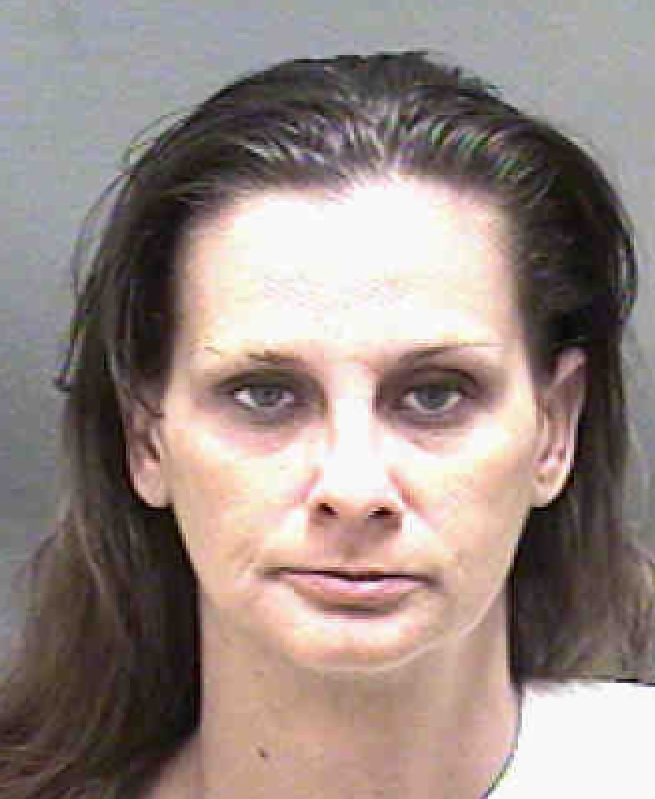
\includegraphics[width=1.0in,height=1.0in]{M_34_W.png}
	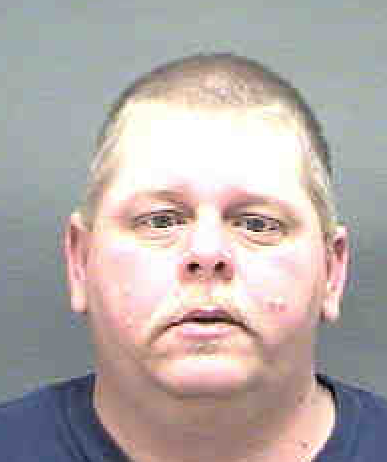
\includegraphics[width=1.0in,height=1.0in]{M_37_W.png}
	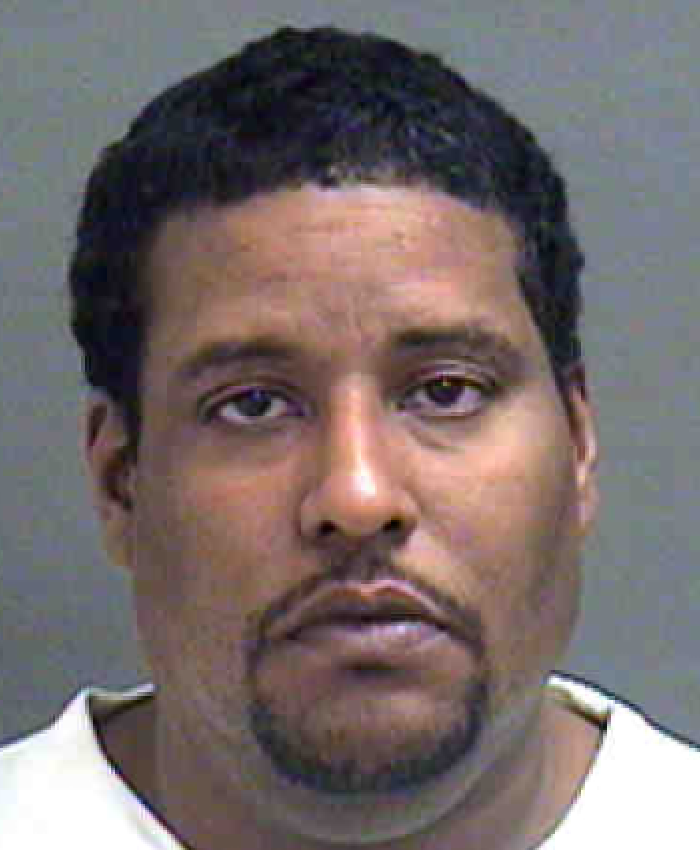
\includegraphics[width=1.0in,height=1.0in]{M_40_B.png}
	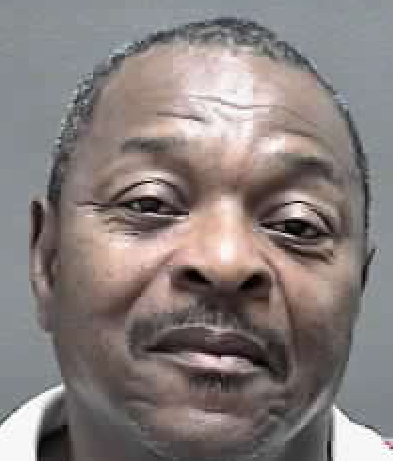
\includegraphics[width=1.0in,height=1.0in]{M_58_B.png}
	}
	\subfigure[celeA数据示例]{
	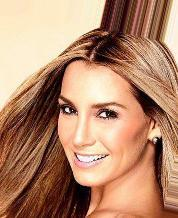
\includegraphics[width=1.0in,height=1.0in]{000001.jpg}
	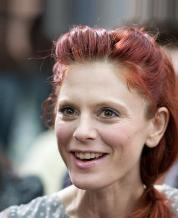
\includegraphics[width=1.0in,height=1.0in]{000002.jpg}
	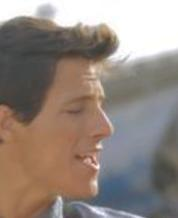
\includegraphics[width=1.0in,height=1.0in]{000003.jpg}
	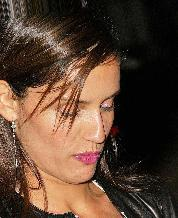
\includegraphics[width=1.0in,height=1.0in]{000004.jpg}
	}
	\subfigure[LFWA数据示例]{
	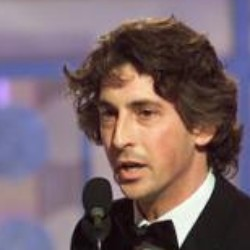
\includegraphics[width=1.0in,height=1.0in]{lfw1.jpg}
	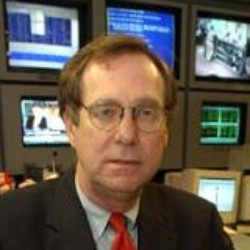
\includegraphics[width=1.0in,height=1.0in]{lfw2.jpg}
	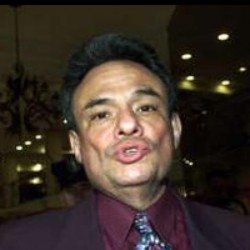
\includegraphics[width=1.0in,height=1.0in]{lfw3.jpg}
	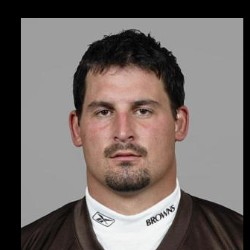
\includegraphics[width=1.0in,height=1.0in]{lfw4.jpg}
	}
	\subfigure[Chalearn LAP and FotW数据示例]{
	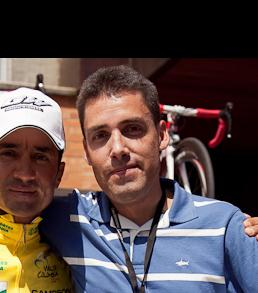
\includegraphics[width=1.0in,height=1.0in]{lap00001.jpg}
	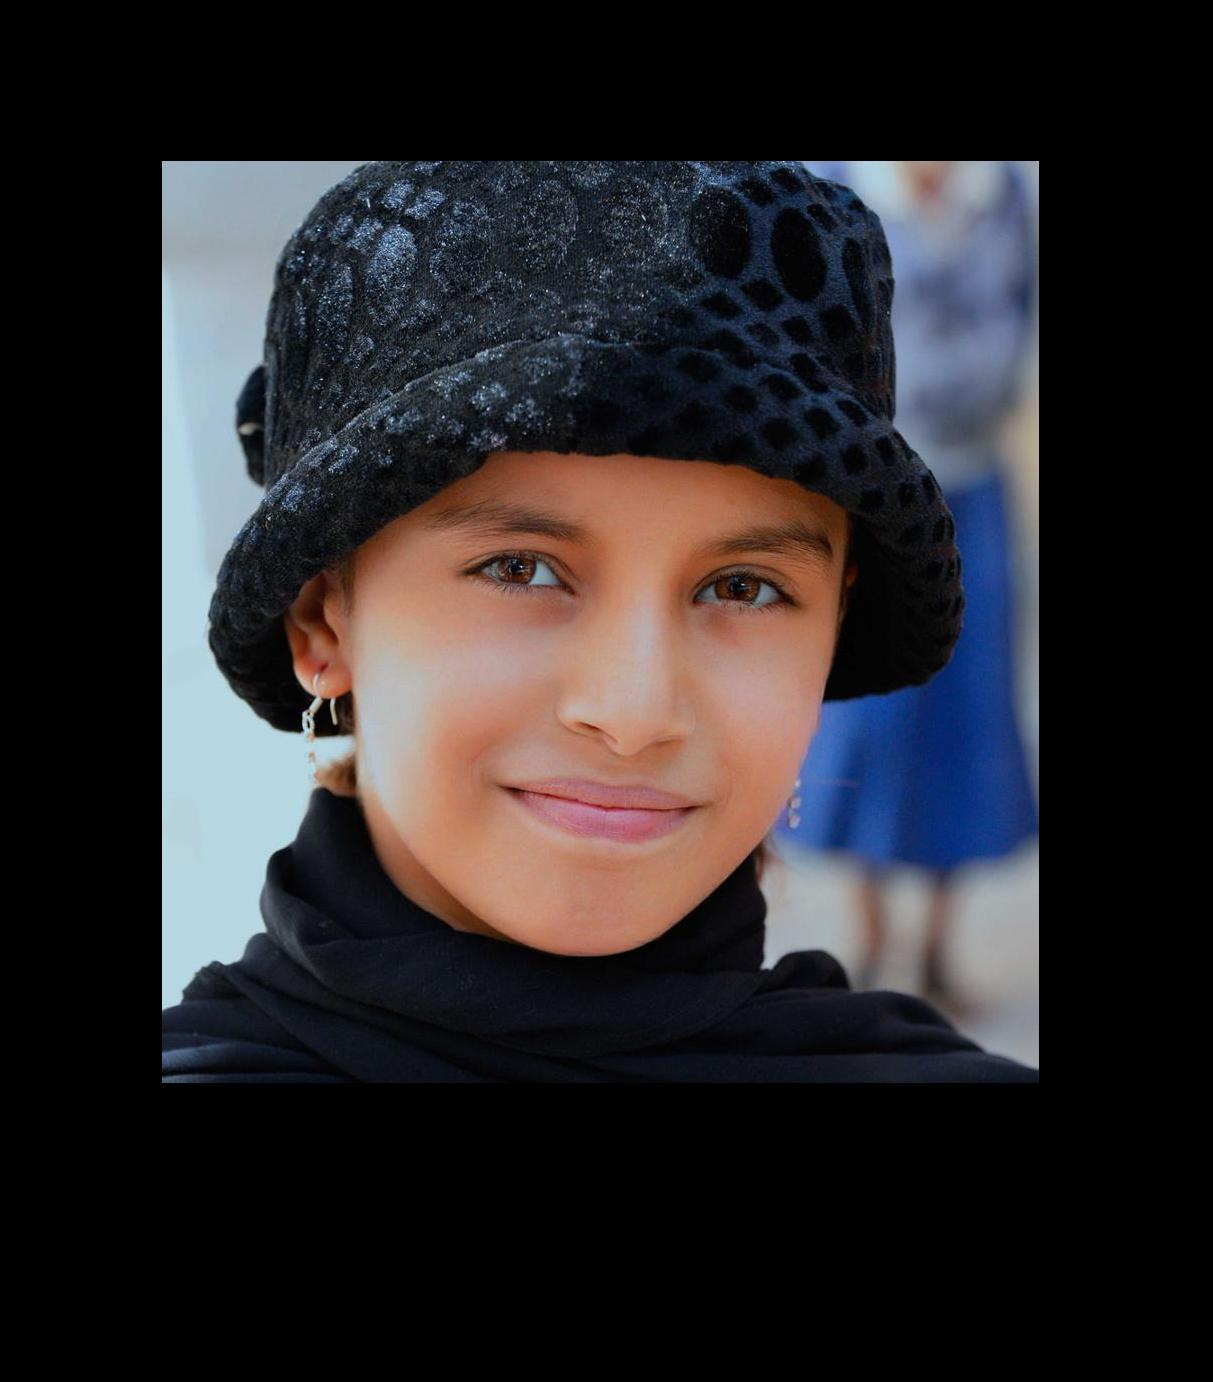
\includegraphics[width=1.0in,height=1.0in]{lap00002.jpg}
	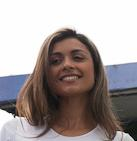
\includegraphics[width=1.0in,height=1.0in]{lap00003.jpg}
	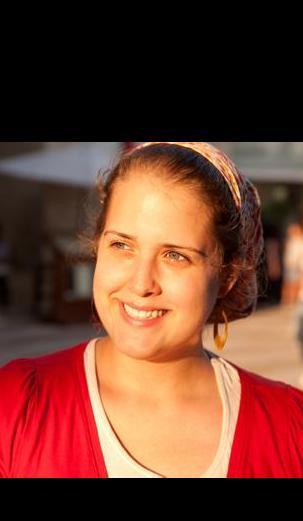
\includegraphics[width=1.0in,height=1.0in]{lap00004.jpg}
	}
	\subfigure[LBS数据示例]{
	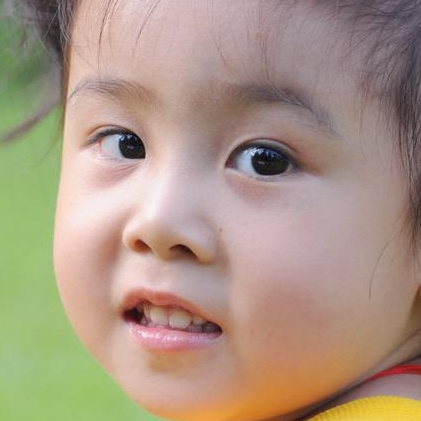
\includegraphics[width=1.0in,height=1.0in]{lbs0.jpg}
	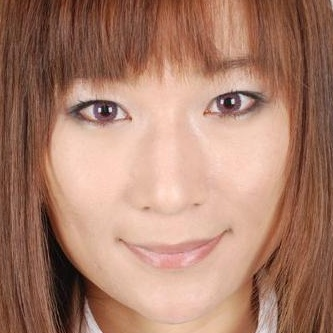
\includegraphics[width=1.0in,height=1.0in]{lbs1.jpg}
	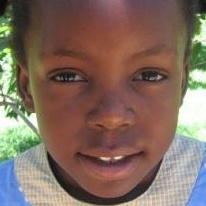
\includegraphics[width=1.0in,height=1.0in]{lbs2.jpg}
	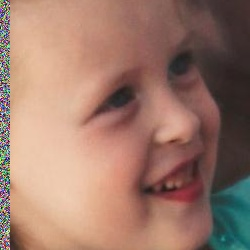
\includegraphics[width=1.0in,height=1.0in]{lbs3.jpg}
	}
	\caption{数据集图片示例}
\end{figure}

这些数据库可以根据所使用的注释方法分为三类:(i)具有序性标签的数据库(MORPHII和LFWA),(ii)具有二进制属性的数据库(CelebA,LFWA)和(iii) 具有单个属性的数据库LAPAge2015和LBS数据库。 我们可以看到,除了MORPH II数据库,其他数据库主要包含真实场景下的人脸图像。  

可以看到人脸属性的数据集其实比较庞大,如果都能够充分利用,可以获得相比于单一数据集更加出色的识别效果。但是每个数据集之间的数据不同、数量不同、标注不同,实际使用中往往使用先训练一个再训练一个的流程,非常耗时而且不能够保证模型效果在原有数据集上保持良好的效果。实际使用来看,使用celeA训练的数据对于lfwA的数据效果并不好,而加入lfwA的数据训练就可以提升相关lfwA上的准确率。但需要注意的是LFWA的数据量远小于celeA的数据量,简单的把两个数据合起来训练,两个数据库之前的差异分布其实并不能得到特别好的弥补,训练的准确率还是不能和单独使用lfwA相比。

类似的问题对于年龄这一属性更严峻一点,不同的数据库标注是不一样的,在morph中是连续的标签,但是在Adience数据集上,年龄的标注是7个单独的类别,如果强行进行label的转换就会存在很多不匹配的现象,无法对其进行测试,但根据Adience重新finetune,那么就会存在类似的数据匹配和模型输出改变的问题。

\section{基于传统特征的人脸属性识别}
基于传统特征的人脸属性识别\cite{HUHAN}往往采用特征提取和分类器结合的方式,其中较为经典的是基于DIF特征的人脸属性识别是经典的属性学习方法,在morphII上一度取得了非常优秀的实验结果,基本框架概述如下:

前端为特征提取阶段,旨在提取对属性有判别力的特征,而不是完全无监督的。后端连接一个层级式的分类器,用于属性学习。具体结构见下图:
\begin{figure}[!ht]
 \centering
	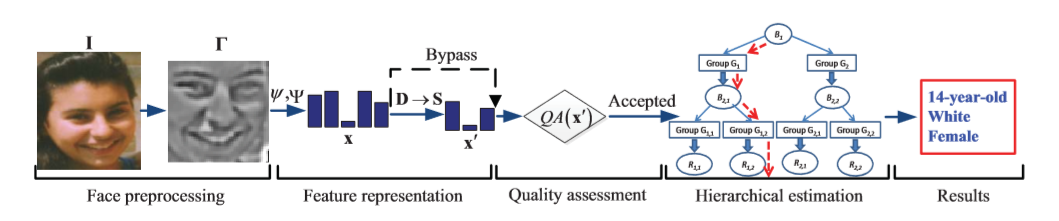
\includegraphics[width=5.0in]{huhanSTLMorph.png}
	\caption{基于DIF特征的人脸属性识别}
\end{figure}

其中有两个主要部分:DIF(Demographic informative features)特征提取,层级式分类器。

1)DIF特征:

DIF(Demographic informative features)是基于BIF(生物启发式特征)的。
比如,输入一个人脸部件,先用Gabor滤波器提特征(12个尺度,8个方向),再做一些池化操作,以减小特征图的数目和维度(6个尺度,8个方向),将得到的特征串成一个4280维的长向量,用来做之后的分类等任务。总体上还是一个无监督的特征处理方法。所以之后,又对此工作做了改进,旨在不仅能够抓住图像细节,还能减小冗余性,提高特征与最终识别任务的相关性。这一部分主要引入一些特征学习工作,从之前的特征集中不断特征子集,挑选出最相关的特征,比如:学习一个新的特征子空间(如LDA),基于Boosting的特征选择。

2)层级分类器的建设:

层级分类器主要针对年龄。比如,首先进行年龄组分类(针对数据集设定阈值),在此按是否超过18岁分为两类;低于18岁的一类再判断是否低于7岁,再分为两类,然后低于7岁再进行回归得到具体的年龄数值,以此类推,先一层一层地通过多个分类器树形展开得到具体的人脸年龄段,然后在具体的人连年龄分段中及进行回归。hu的实验证明,这种层级式的分类方式要优于直接分类方法。

基于DIF特征的属性识别方法是经典的基于传统特征和分类器的属性识别方法,即使在现在,特征融合、层级分类器建设等操作依然具有一定的借鉴意义

问题与不足:尽管效果不错,但整个方法还是有很多的问题,例如,层级分类器确实能够提升分类的效果,但是复杂都明显过高,并不简洁,使用基于传统滤波器和表层信息的图像特征,需要大量的特征筛选和过滤工作。而且总结来讲是DIF系统还处在各个部分的分开设计,整个系统并不是处在一个整体性学习的状态。需要较多的人工干预和训练才能得到较好的效果。
\section{基于共享神经网络特征和最大间隔分类器的人脸属性识别}
随着深度学习方法的提出,深度学习的特征慢慢取代了传统的手工设计的特征,结合深度学习中经常使用的分类器,得到了更高的效果。
具有代表性的是基于级联CNN网络和SVM分类器的识别方法,使用两个CNN框架Lnet和Anet进行级联学习,其中Lnet负责检测图片中的人脸,Anet针对于Lnet中检测人脸使用交叉熵loss进行训练,为了提升识别的准确性使用SVM对于ANet中的特征进行训练。最后由SVM分类器输出具体的人脸属性预测值。
其中不难发现器图片的标签就采用的是标签化编码的方式。
\begin{figure}[!ht]
 \centering
	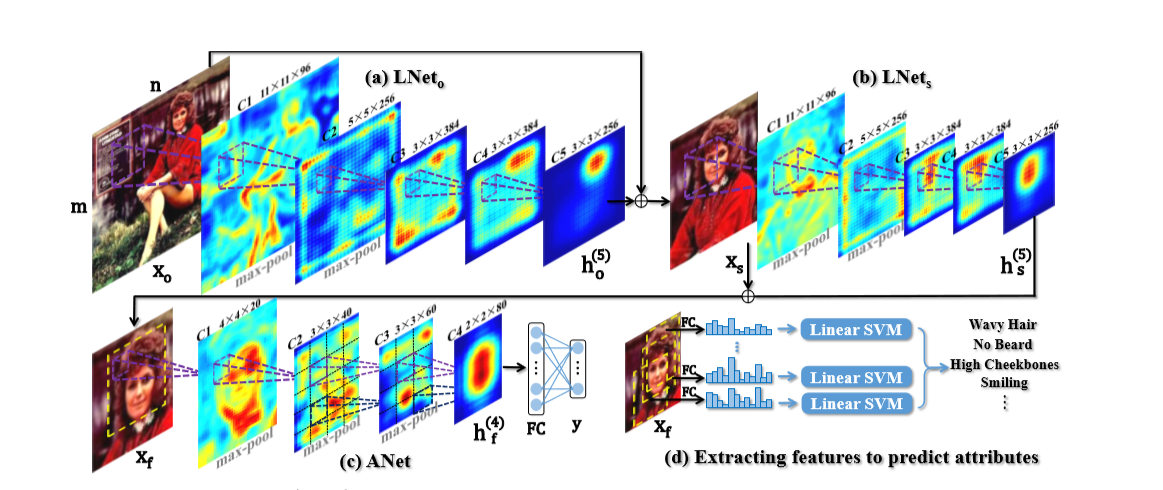
\includegraphics[width=6.0in]{liuziwei.png}
	\caption{基于共享神经网络特征和SVM分类器的人脸属性识别}
\end{figure}

问题与不足:其实在训练的过程中,神经网络就已经可以对于属性进行预测,但是识别的效果却并不如SVM训练的结果,说明在这一框架中,神经网络对于不同属性的自网络决策层和loss函数设计的不够好。从图中可以看到,不同的人脸属性之间都是用的同样的FC层全连接而来的。不能够体现出属性整体和局部特性。
\section{基于共享特征和子任务模块的端到端的人脸属性学习}
机器学习神经网络中的端到端,一般是指输入原始数据,输出最后结果的过程。对于人脸属性的识别过程来讲:如何解决人脸属性多任务的输出是解决问题的关键,目前比较主流的方法是使用网络共享单元和网络子任务模块相互组合的方式\cite{HUHAN_MTL},具体来讲可以参考下图:
\begin{figure}[!ht]
 \centering
	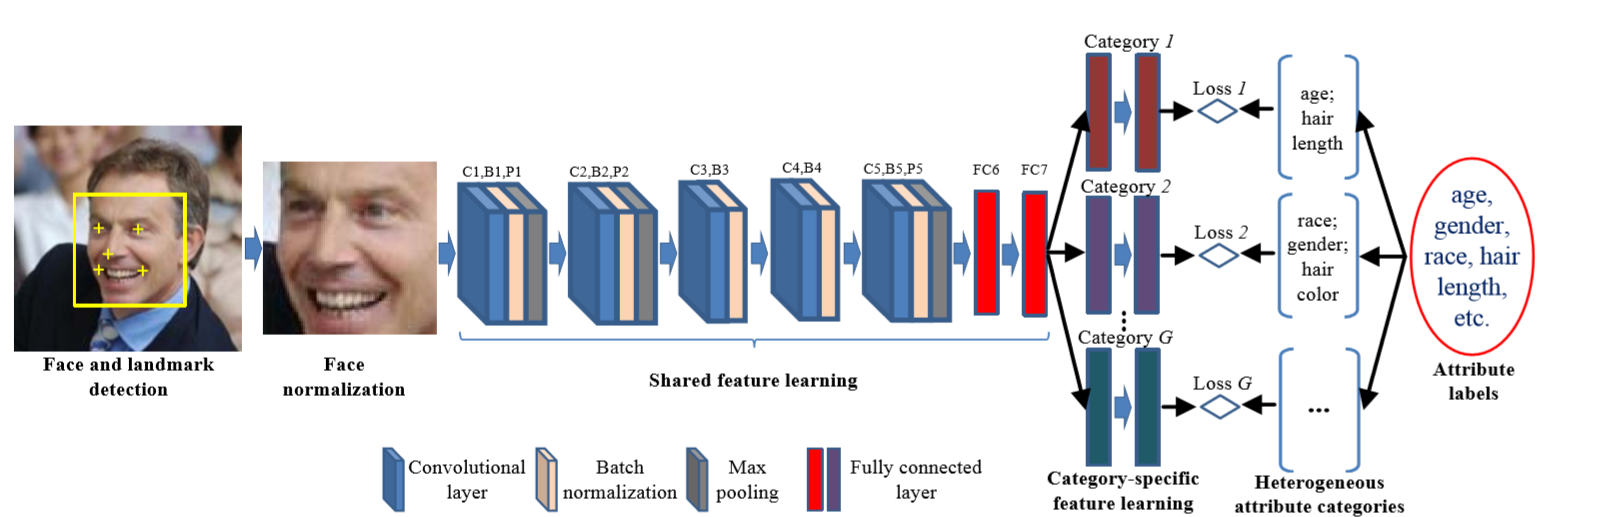
\includegraphics[width=6.0in]{huhanMTL.png}
	\caption{基于端到的人脸属性学习}
\end{figure}
对于不同的人脸识别任务,如果希望能够在一个框架中通过端到端的方式解决,而且具有一定可用性,就需要将不同属性识别任务中重复性学习的工作整合成共享模块,然后不同的人脸属性模块再基于共享模块单独对于自身的学习任务单独进行学习。端到端基于共享模块的学习方法可以很大程度上加快过程中的使用效率,同时简化了训练流程。而类别特定的子模块学习旨在对共享特征进行精细调整,以便对每个异构属性类别进行最优估计。 由于有效的共享特征学习和类别特定的特征学习,基于共享单元和网络子任务模块的方式在保持低计算代价的同时,实现了更高精度的属性估计精度,使其在许多人脸识别应用中具有价值。

问题与不足:基于共享模块和子网模块的识别方式虽然看上去简化了识别的过程,但却是以减少了模型训练的先验规则为代价。也就是说把更多的学习过程交给了模型本身,那么模型的学习过程一方面取决于模型自身设计的学习能力和使用的训练方法,而更重要的是训练数据的选择和实用。

尤其对于端到端网络来讲,由于整体网络结构变得封闭和训练方式的固定化,训练数据的选择和训练过程中对于真实环境的模拟就变得尤为重要。但真实场景中的数据具有较大的变化,包括数据的场景来源不同,数据中样本的比例不均匀,数据自身的姿态和角度变化等。训练样本的选取和预处理过程成了和网络结构选择一样重要的问题。
\section{使用SA-sfotmax进行模型稳定化输出}
模型的稳定性输出体现在很多方面,如常见的连续变化的视频,不同设备收集的图像等。在这些场景中,网络可能偶尔会发生判断错误的情况,影响用户的体验。虽然很多时候可以采用平滑的策略进行弥补,但是网络本身的稳定性性能是整个识别系统的关键。
为了提升属性识别模型的稳定化输出,我提出了基于带有自评功能的softmax(Self-assessment softmax SA-softmax),以及相应的动态标签(Dynamic tag,Dt)训练方法来增强网络的稳定性。
\subsection{SA-softmax}
传统的softmax with loss 面对N个输入类别,或有N元数字作为输入,同时输入的标签是从0~N-1的一个整形数字用以表示具体的ground truth。通过softmax操作,计算出每个类别的相对概率值。
将对应标签的概率输出取负对数作为损失函数和优化的对象。

SA-softmaxLoss在分类结果上将网络分类概率输出由N个,改为N+1个,第N+1维值定义为无法识别类(unrecognizable class)。分类label由原来的一元数字标签变为一个四元的整形数组分别用于储存图片在过去训练过程中出现的次数、图像被判正确的次数、图像真实的标签,图像目前的标签。训练的过程中使用动态标签(Dynamic tag,Dt)训练方法,不断更新训练图片的类别。

测试的过程中,首先使用softmax对于所有N+1类求出无法识别类的概率输出,使用1-无法识别类的概率作为网络的置信输出。
根据置信度对照表给出网络置信度评价,对其余的类别重新使用softmax进行概率获取。最后的输出形式是:输出类别概率+网络置信度概率。
 \begin{table}
  \centering
   \caption{SA-softmax的置信度判断对照表}
   \label{tab:req-pkg}
   \begin{tabular}{c|c}
     \toprule
     网络置信度 & 模型自评描述 \\
     \midrule
     S:80-100 & 判定模型输出非常自信				 	\\
     A:60-80  & 判定基本正确 				 		\\
     B:40-60  & 判定可以猜测 但不对结果负责  	 	\\
     C:20-40  & 判定难以识别    					\\
     D:0-20   & 判定完全无法识别				\\
     \bottomrule
   \end{tabular}
 \end{table}
\subsection{动态调整标签的训练方法}
对于softmax简单的加入一类未知类,还远远不够,至少训练的样本都没有,这分支的梯度永远都是0,不会对网络产生训练作用。但实际上训练开始的时候我们是无法知道哪些图片是网络不能够正确识别的,所以引入动态调整标签的训练方法:
于是在现有的框架下,我们设计了如下的训练方法:

\begin{algorithm}[h]
\caption{动态标签调整的算法流程}
\begin{algorithmic}[1]
\STATE 首先不加入SA-softmax,将分类网络训练至收敛。
\STATE 将训练收敛的网络模型的softmax改成SA-softmax。
\WHILE {模型收敛 or 达到训练次数}
\FOR{epoch $i \in [0,9]$} 
\STATE 更新训练图片的标签四元组中的出现次数和判断正确次数。
\ENDFOR
\IF{图片现有标签和实际标签是否一致}
\IF{训练10次准确率高于0.5}
\STATE 不对标签进行修改,说明被模型对该图片训练良好。
\ELSE[准确率低于0.5]
\STATE 将图片标签标记成N+1,说明网络无法将其良好训练。
\ENDIF
\ELSE 
\IF {准确率高于0.5}
\STATE 不对标签进行修改,这类图片被成功分到N+1类,模型自评成功。
\ELSE [准确率低于0.5]
\STATE 改回原来的标签,说明依然并不能将其分类,应当重新观察。
\ENDIF
\ENDIF
\STATE 清空出现次数和被判断正确的次数
\ENDWHILE
\end{algorithmic}
\end{algorithm}

\section{实验设置}
在上一节中,总结了在人脸属性任务的主流方法和发展过程,可以看出随着深度学习的发展和端到端学习在模式识别过程中的发展,很多问题都得到了改善,但依然存在着一些主流问题和场景困境一直存在,我仔细对于相关问题进行了思考总结。
\begin{enumerate}
\item 问题一:人脸数据库的标注各不相同,使用怎样的框架才能将不同的数据库都充分利用起来。
\item 问题二:使用怎样的数据输入和数据处理方式和训练方式,才能发挥深度学习的特性。
\item 问题三:提高模型输出的稳定性,减轻网络错误输出的偶然性和影响。
\end{enumerate}
针对于于问题的不同种场景分别设计任务和实验进行验证和训练网络优化。具体介绍如下:
\subsection{网络结构和训练环境}
在本文中,所有的网络结构都以改进版的Alexnet为基础,进行训练。具体网络结构细节包括:
Alexnet的基础结构包括:5层卷积,5层pooling,2个全连接层;
每个卷积层后面都加入BatchNorm层,所有的激活函数都是用relu,将原来的卷积扩充为ConvUnit;
所有的pooling都采用kernel 为3*3,步长为2的Max pooling;
除此之外在最后层的pooling输出,不同的任务会采取不同的subnet结构作为训练任务的分支,这在不同的实验中会一一说明。

输入人脸图片以人脸检测输出的正方形人脸框为基础,输入大小都为256*256。在训练属性之前,将网络在人脸识别的数据中进行了预训练。实验数据中使用了两台拥有4块nvidia-GTX1080显卡的机器,使用caffe和mxnet\cite{MXNET}进行了相关训练,包括在一些任务上的分布式的多机多卡训练。

下面给出关于多机多卡训练的网络结构示意图:
 \begin{figure}[!ht]
 \centering
	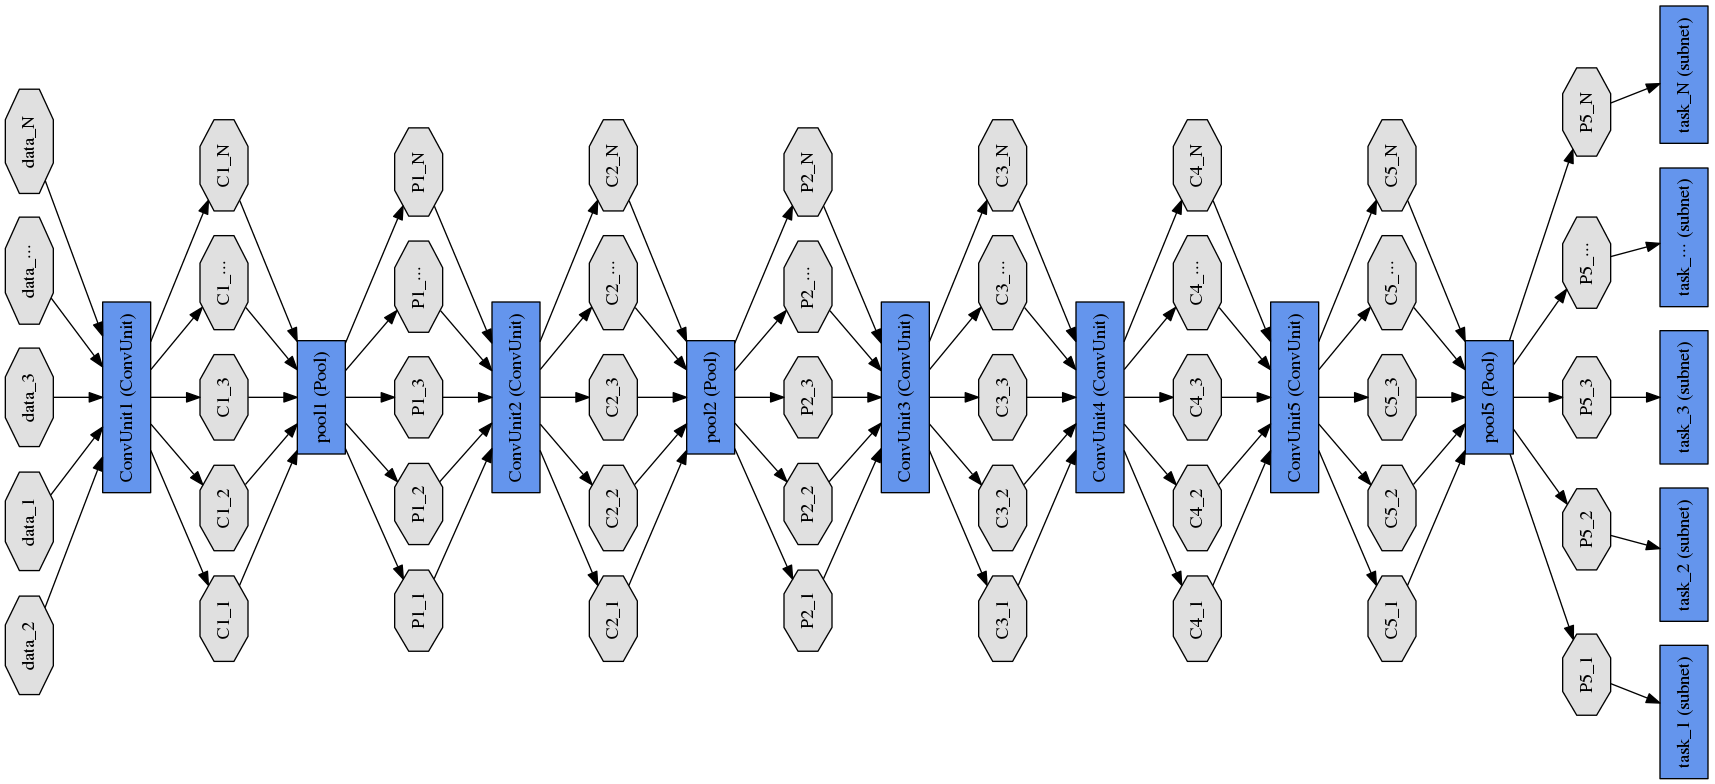
\includegraphics[width=6.5in]{tri_TB.png}
	\caption{数据集并行的网络结构}
\end{figure}
关于超参数的选择学习率使用multi-ste的方式进行训练,前50000轮学习率设置为0.001,
之后每100000轮降低0.1,weightdecay设置为0.00005。momentum设置为0.9.

\subsection{数据集并行训练的方式改进问题一}
对于不同的数据集来讲,预处理的方式往往类似,也就是说输入图片虽然不同,但是输入的格式是一致的(事实上即使不同也没有什么问题,关键是图片数据不同),但是因为标签不同,导致在一个网络结构中无法进行统一的训练。
那么不妨就按照多个单独的网络对于图像进行训练,每个网络在特征提取阶段采用相同参数的全卷及网络结构进行特征提取,但每一层的特征图会单独进行存储,训练的时候每个数据集都按照自己的数据结构特性为了拟合loss层的设计,采用不同的子网络结构。	
在这一过程中需要使用上一节提到的多机多卡的技术,不同的单机多卡并不能满足实验对于计算资源的需求。而如果为了训练采用batchsize较小的策略,往往不能够取得良好的效果。

为了验证这方案的有效性,我们使用两个数据集Morph和LBS数据集作为联合训练输入,Morph种年龄的标签按照0~100的有序性分布,
而在LBS数据中,年龄是无序性的分成了5个类别,为此单独为此单独设计了相关的子网络模型,其子网络结构分别设计如下:
 \begin{figure}[!ht]
 \centering
	\subfigure[针对于LBS的无序性5类年龄标签子网络结构]{
	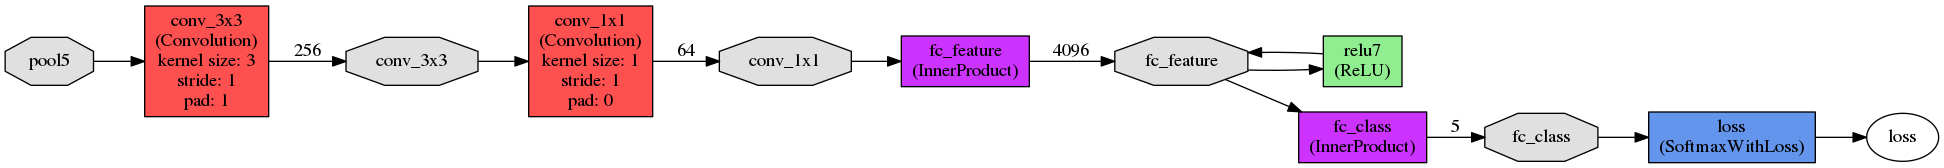
\includegraphics[width=5in]{subnet_class.png}
	}
	\subfigure[针对于Morph的0~100的有序性标签子网络结构]{
	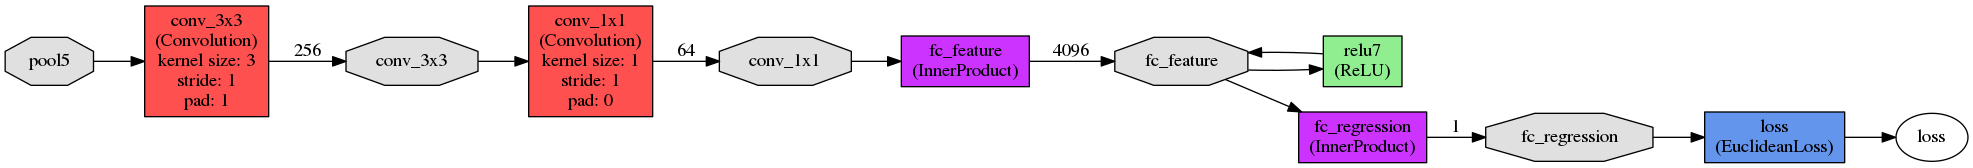
\includegraphics[width=5in]{subnet_reg.png}
	}
	\caption{数据集并行的网络结构}
\end{figure}

其中3x3的子网络是为了学习共享特征图中的信息,1x1的卷积是为了减少计算量,fc\_feature为了提取相关任务特征,fc\_class/regression是对应结果的表示形式。

测试方法对于回归的年龄数值使用MAE(mean absolute error),对于分类的年龄使用Precision来衡量性能:

\begin{equation}{
\begin{split}
& MAE=\frac{\sum_{i=1}^{n} \left | y_i-x_i \right |}{n}  \\
& Presion=\frac{N_{tp}}{N}
\end{split}
}\end{equation}

经过训练可以得到具体的实验结果可参见下表:
 \begin{table}[!h]
  \centering
   \caption{在Morph和LBS上的准确率结果}
   \label{tab:req-pkg}
   \begin{tabular}{c|c|c|c}
     \toprule
     训练方式&MorphII& LBS& Morph和LBS并行训练\\
     \midrule
     Morph II上的MAE(绝对误差)&4.2  &NA & 3.5 \\
     LBS上的 Presion(百分比)&NA  &82.9& 85.2\\
     \bottomrule
   \end{tabular}
 \end{table}

\subsection{人脸矫正固定输入格式改进问题二}
在很多人脸任务中,由于人脸是一个基于模板的识别对象,所以对于固定空间分布有着一定的要求,直接检测的人脸对于人脸属性的任务很多时候效果不佳,这一问题在人脸识别的相关算法上已经有所受体现,那么使用人脸矫正的相关与处理方式可以很好地解决人脸对于固定空间分布的要求,具体经常采用的方式是根据人脸landmark点的人脸alignment处理:

在得到人脸五个位置的关键点即左眼眼球中心、右眼眼球中心、鼻尖、最左角和右嘴角之后,
通过计算五点与标准脸五点之间的仿射变换矩阵,之后将图片中所有点与仿射变换矩阵相乘,得到了经过放射变化的图像,通过简单的截取可以得到对应的矫正之后的图像。
实验中标准脸大小为450x450,其中五个点的中心坐标分别为:
(200.0,260.0)、 (288.0,260.0)、 (244.0,488.0)、 (206.0,370.0)、 (282.0,370.0),矫正效果:
\begin{figure}[!h]
 \centering
	\subfigure[人脸矫正之前的图像]
	{
	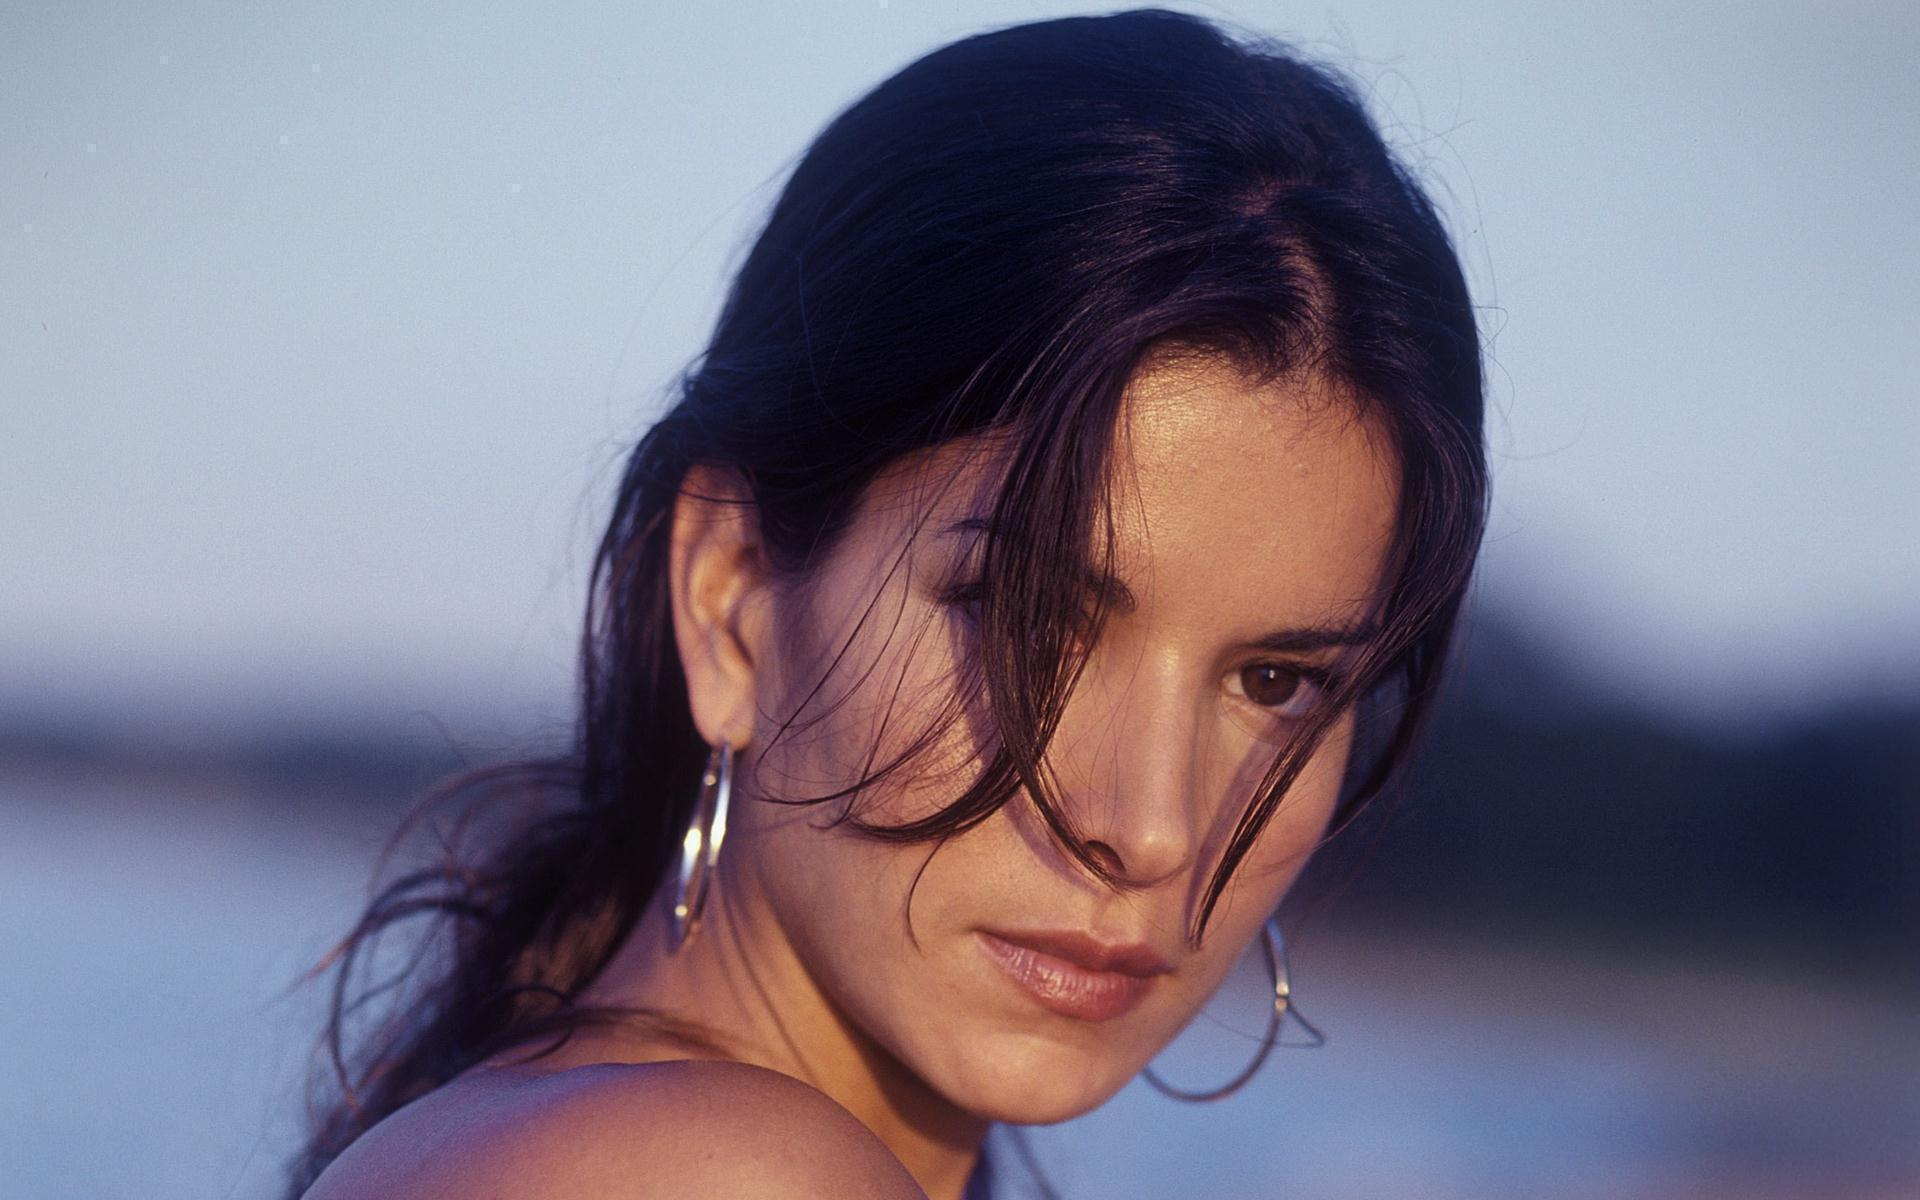
\includegraphics[height=1.50in]{beforealign.jpg}
	}
	\subfigure[人脸矫正之后的图像]{
	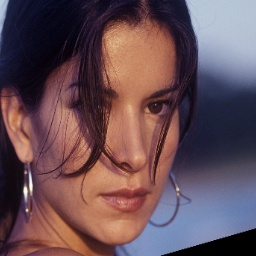
\includegraphics[width=1.50in]{align.jpg}
	}
	\caption{人脸矫正效果演示}
\end{figure}

针对于人脸矫正对于训练的影响主要使用了Chalearn数据集中的性别和微笑属性作为任务目标,为了验证实验效果没有使用上一步中数据并行的策略。只是简单的式使用了基本的alexnet结构,输入的图片处理方式不同。单独训练两个网络,最后得到准确率结果如下:
\begin{table}[!h]
  \centering
   \caption{在Chalearn数据集上的性别和微笑准确率结果}
   \begin{tabular}{c|c|c}
     \toprule
     测试集&性别准确率&微笑准确率\\
     \midrule
     人脸框直接输入  & 84.5 & 81.4 \\
	 人脸矫正后输入  & 89.9 & 84.3 \\
     \bottomrule
   \end{tabular}
\end{table}
\subsection{网络自评估模块改进问题三}
在这一模块中,依然选取了LBS数据集中的年龄5类作为训练和验证的测试集,依然基于基本的Alex网络结构,子网络模块会分别使用softmax和SA-softmax。

主要比照过程,是使用普通softmax训练的得到的人脸年龄准确率,和加入SA-Softmax训练策略之后网络整体性能对于,以五类年龄分类的top1准确率作为评价指标。
但值得注意的是,由于自评模块的输出和正常的输出不一致,所以使用简单的准确率进行评判其实并没有完全利用自评网络模块的结果输出,我们通过自评模块置信度对照表,对于不同区间的网络准确率进行计算,并且统计各个区间之间图片的图片出现次数。一一和普通网络的输出的准确率进行对照,得到结果如下:
\begin{table}[!h]
  \centering
   \caption{在LBS数据集上的性别准确率结果}
   \begin{tabular}{c|c|c}
     \toprule
     置信分段&年龄分类准确率&测试图片数目\\
     \midrule
      正常训练 &  85.2 & 20000 \\
	  自评训练 &  93.1 & 20000 \\	  
      S        &  95.9 & 15575 \\
	  A        &  88.8 & 2830 \\
	  B        &  80.1 & 1031 \\
	  C        &  77.8 & 384  \\
	  D        &  30.9 & 180  \\
     \bottomrule
   \end{tabular}
\end{table}

\section{实验结论与分析}
从实验的结果来看:
\begin{enumerate}
\item 数据集并行训练的方式进行训练的过程之中,经过并行训练的数据集得到的模型在morph上MAE误差减少了0.7。也就是说减少18\%的误差,而在LBS数据集的测试上准确率提升了2.3%,减少了13%的误差。可以看到联合训练的方式能够起到增加训练数据的效果,在不同的数据集中都取得了很好的提升。

可以看到联合训练的方式能够起到增加训练数据的效果,在不同的数据集中都取得了很好的提升。而且得益于联合训练的结构特性,可以在一个模型中输出两种数据格式的预测值,也就是年龄的回归值和分类值,相比于原本每种数据格式都需要重新训练的方式更见简洁。


\item 对于问题二,使用人脸矫正的图片可以提高人脸性别和微笑的识别效果,对于性别任务来讲任务从准确率84.5提升到89.9,错误率减少了34.8\%,
微笑的准确率从81.4提升到84.3,错误率减少了15.5\%。

说明在使用人脸矫正的方法情况下,可以提升对于微笑和性别的识别准确率。但是和原本的直接将人脸检测的图片框截取的图片作为输入的方式,人脸矫正的处理方式则稍显复杂,而且还在一定程度上取决于人脸landmark的效果。而且仔细分析来看,对于微笑任务的识别效果提升并不如人脸性别的识别效果提升。说明人脸矫正的策略可能并不是所有的人脸属性任务都会具有相同的效果,比如人脸姿势和角度相关属性,通过矫正甚至可能改变人脸属性。

但是人脸属性矫正还是作为当年最流行的人脸任务与处理方式,在大多数任务中被证明有效。
\item 
对于问题三,自评网路对于人脸年龄的识别有比较明显的提升,对于使用普通softmax和SA-softmax的不同策略的模型,使用自评网络训练的方法将人脸年龄5分类的top1准确率从85.2提升到93.1,效果显著。
而具体来看,有15575张图片的置信度为S级,而且S级的人脸准确率达到95.9\%。而评级为A的图片数量为2830,准确率为88.8\%。其余评级的准确率都比正常训练要低。也就是说有92.0\%的图片可以通过自评模块获得比正常训练更高的准确率。这也正是自评网络的优势所在,能够提升系统的整体判断准确率。从而减少人工审核的工作量。
\end{enumerate}

\section{本章小结}
在本章中,我们通过对于人脸属性和性质的分析,不同人脸属性的数据库简介。以及人脸属性中的常见做法的分析和介绍。逐步分析了人脸属性中面临的问题。

在设计人脸属性是别的方案过程中,增加BN和自网络模块,以神经网络为基础设计人脸属性的识别模型。对于具有不同标签的人脸属性的数据,共享基础结构,单独设计自网络模块的方式并行训练,并采用多机多卡的方式加速训练。而对于人脸属性中输入格式形式,使用经典的基于landmark的形式进行人脸矫正。最后为了稳定网络的输出,我们为网络加入具有自评估能力的SA-softmax,不仅提高了人脸的属性识别的准确率,同时增加了模型对于自身能力的评估能力。









 
 
 